\documentclass[10pt]{beamer}

\usetheme[progressbar=frametitle, numbering=fraction,]{metropolis}

\usepackage{booktabs}
\usepackage{pgfplots}
\usepgfplotslibrary{dateplot}
\usepackage{texshade}      
\usepackage{amsmath}
\usepackage{amssymb}
\usepackage{xspace}
\usepackage{xcolor}
\usepackage{appendixnumberbeamer}
\usepackage{multirow}
\usepackage{verbatim}

\usepackage{tikz}
\usetikzlibrary{shapes.geometric, arrows}
\tikzstyle{startstop} = [rectangle, rounded corners, minimum width=3cm, minimum height=1cm,text centered, draw=black, fill=red!30]
\tikzstyle{io} = [trapezium, trapezium left angle=70, trapezium right angle=110, minimum width=3cm, minimum height=1cm, text centered, draw=black, fill=blue!30]
\tikzstyle{process} = [rectangle, minimum width=3cm, minimum height=1cm, text centered, draw=black, fill=orange!30]
\tikzstyle{decision} = [diamond, minimum width=3cm, minimum height=1cm, text centered, draw=black, fill=green!30]

\tikzstyle{arrow} = [thick,->,>=stealth]


\newcommand{\themename}{\textbf{\textsc{metropolis}}\xspace}

\setbeamercovered{invisible}
\setbeamertemplate{caption}{\raggedright\insertcaption\par}

\title{Cardiovascular Physiology}
%\subtitle{What we see, is not what it is}
\date{\today}
\author{Saket Choudhary}
\institute{BISC 104\\Session 6}
%\titlegraphic{\hfill
\includegraphics[height=1.5cm]{logo}}

\begin{document}

\maketitle



\begin{frame}[fragile]{Today's Experiment}
\begin{center}
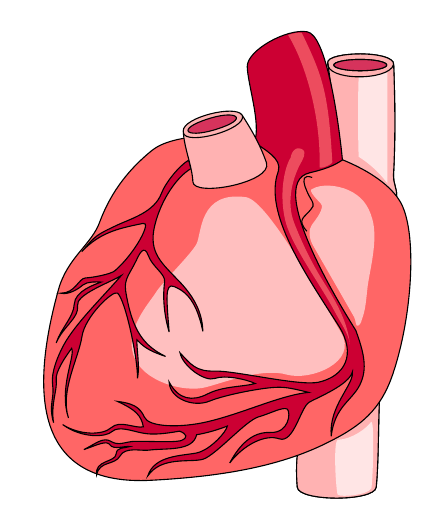
\begin{tikzpicture}[scale=-0.5]
\draw[fill=red!30!white](.456,3.236)
    .. controls (.422,4.168) and (.408,5.095) .. (.461,6.046)
    .. controls (.475,6.228) and (.365,6.400) .. (.379,6.601)
    -- (.819,11.816)
    .. controls (.843,12.194) and (.838,13.389) .. (.900,13.972)
    .. controls (.943,14.340) and (2.870,14.340) .. (2.903,13.972)
    .. controls (2.927,13.699) and (2.932,13.436) .. (2.903,13.169)
    -- (1.847,5.401)
    .. controls (1.914,4.627) and (2.033,3.924) .. (2.129,3.193)
    .. controls (2.177,2.906) and (.441,2.863) .. (.456,3.236) ;
\draw[fill=red!30!white] (.456,3.236)
    .. controls (.422,4.168) and (.408,5.095) .. (.461,6.046)
    .. controls (.475,6.228) and (.365,6.400) .. (.379,6.601)
    -- (.819,11.816)
    .. controls (.843,12.194) and (.838,13.389) .. (.900,13.972)
    .. controls (.943,14.340) and (2.870,14.340) .. (2.903,13.972)
    .. controls (2.927,13.699) and (2.932,13.436) .. (2.903,13.169)
    -- (1.847,5.401)
    .. controls (1.914,4.627) and (2.033,3.924) .. (2.129,3.193)
    .. controls (2.177,2.906) and (.441,2.863) .. (.456,3.236) ;
\draw[fill=red!60!white] (.303,6.697)
    .. controls (-.161,7.442) and (-.022,9.641) .. (.484,11.118)
    .. controls (.795,12.022) and (1.297,12.414) .. (2.062,12.801)
    .. controls (3.429,13.513) and (5.112,13.714) .. (6.598,13.795)
    .. controls (9.495,13.957) and (9.738,11.735) .. (8.974,8.967)
    .. controls (8.744,8.126) and (8.123,7.815) .. (7.917,7.222)
    .. controls (7.683,6.606) and (7.310,5.999) .. (6.598,5.420)
    .. controls (5.570,4.579) and (1.230,5.210) .. (.303,6.697) ;
\fill[fill=red!25!white] (2.540,6.405)
    .. controls (2.296,6.257) and (1.890,6.300) .. (1.608,6.424)
    .. controls (1.274,6.577) and (1.101,6.802) .. (1.001,7.151)
    .. controls (.858,7.652) and (1.025,8.293) .. (1.106,8.795)
    .. controls (1.149,9.072) and (1.149,9.402) .. (1.254,9.684)
    .. controls (1.278,9.746) and (1.278,9.823) .. (1.360,9.870)
    .. controls (1.426,9.909) and (1.412,9.732) .. (1.460,9.651)
    .. controls (1.747,9.144) and (2.210,8.346) .. (2.502,7.834)
    .. controls (2.602,7.657) and (2.631,7.437) .. (2.531,7.303)
    .. controls (2.411,7.146) and (2.206,6.883) .. (2.306,6.768)
    .. controls (2.382,6.682) and (2.621,6.453) .. (2.540,6.405) ;
\fill[fill=red!25!white] (4.204,6.606)
    .. controls (5.413,6.434) and (5.327,7.543) .. (5.466,7.796)
    .. controls (5.599,8.054) and (6.350,8.785) .. (6.498,9.029)
    .. controls (6.646,9.273) and (7.282,9.947) .. (7.067,10.616)
    .. controls (6.847,11.290) and (5.776,11.582) .. (5.212,11.429)
    .. controls (4.643,11.271) and (3.773,10.941) .. (3.166,11.113)
    .. controls (2.559,11.280) and (1.350,10.793) .. (1.790,10.052)
    .. controls (2.225,9.311) and (3.640,6.692) .. (4.204,6.606) ;
\draw[fill=yellow] (1.307,3.107)
    .. controls (1.675,3.107) and (1.976,3.169) .. (1.976,3.250)
    .. controls (1.976,3.327) and (1.675,3.394) .. (1.307,3.394)
    .. controls (.934,3.394) and (.633,3.327) .. (.633,3.250)
    .. controls (.633,3.169) and (.934,3.107) .. (1.307,3.107) ;
\draw[fill=blue!20!red!80!white] (1.307,3.107)
    .. controls (1.675,3.107) and (1.976,3.169) .. (1.976,3.250)
    .. controls (1.976,3.327) and (1.675,3.394) .. (1.307,3.394)
    .. controls (.934,3.394) and (.633,3.327) .. (.633,3.250)
    .. controls (.633,3.169) and (.934,3.107) .. (1.307,3.107) ;
\fill[fill=red!10!white] (1.024,14.000)
    .. controls (.991,13.929) and (.924,12.146) .. (1.039,12.323)
    .. controls (1.120,12.452) and (1.498,12.753) .. (1.870,12.767)
    .. controls (2.004,12.777) and (1.918,14.129) .. (1.875,14.163)
    .. controls (1.789,14.230) and (1.110,14.173) .. (1.024,14.000) ;
\fill[fill=red!10!white] (.618,3.432)
    -- (.618,6.247)
    .. controls (.852,5.941) and (1.086,5.745) .. (1.345,5.578)
    .. controls (1.364,5.033) and (1.368,4.125) .. (1.345,3.556)
    .. controls (1.096,3.556) and (.862,3.518) .. (.618,3.432) ;
\draw[fill=white] (4.872,5.215)
    .. controls (4.944,5.607) and (4.891,5.884) .. (4.595,6.061)
    .. controls (4.389,6.185) and (3.749,6.013) .. (3.864,5.664)
    .. controls (3.974,5.339) and (4.088,5.081) .. (4.346,4.923)
    .. controls (4.533,4.813) and (4.858,5.119) .. (4.872,5.215) ;

\draw[fill=red!80!blue] (5.662,5.665)
    .. controls (5.643,5.732) and (5.624,5.803) .. (5.604,5.880)
    .. controls (5.944,6.076) and (6.355,6.640) .. (6.522,7.314)
    .. controls (6.699,8.031) and (6.336,8.284) .. (5.853,8.796)
    .. controls (5.523,9.154) and (5.313,9.541) .. (5.303,10.014)
    .. controls (5.485,9.106) and (5.844,8.958) .. (6.030,8.877)
    .. controls (6.278,8.767) and (6.221,9.221) .. (6.159,10.029)
    .. controls (6.341,9.412) and (6.298,8.944) .. (6.274,8.752)
    .. controls (6.245,8.561) and (6.589,8.370) .. (6.685,8.093)
    .. controls (6.799,7.777) and (6.924,8.069) .. (6.991,8.208)
    .. controls (7.153,8.547) and (7.311,8.681) .. (7.263,8.987)
    .. controls (7.096,10.033) and (6.780,10.387) .. (6.250,10.650)
    .. controls (6.728,10.492) and (6.833,10.373) .. (6.976,10.230)
    .. controls (6.991,10.440) and (6.900,10.870) .. (6.962,11.209)
    .. controls (6.957,10.669) and (7.277,9.197) .. (7.469,9.044)
    .. controls (7.579,8.953) and (8.296,9.632) .. (8.372,10.139)
    .. controls (8.458,10.698) and (8.936,11.535) .. (8.716,12.213)
    .. controls (8.970,11.458) and (8.535,10.636) .. (8.635,10.445)
    .. controls (8.778,10.641) and (9.060,11.037) .. (9.027,11.257)
    .. controls (8.994,11.477) and (9.170,11.874) .. (9.094,12.333)
    .. controls (9.228,11.883) and (9.065,11.702) .. (9.118,11.377)
    .. controls (9.166,11.052) and (8.979,10.626) .. (8.836,10.359)
    .. controls (8.549,9.828) and (7.889,9.187) .. (7.373,8.595)
    .. controls (7.708,8.796) and (8.535,9.077) .. (8.487,9.369)
    .. controls (8.434,9.661) and (8.860,9.900) .. (9.027,10.306)
    .. controls (8.903,9.928) and (8.587,9.656) .. (8.568,9.321)
    .. controls (8.554,8.982) and (8.023,8.815) .. (7.889,8.762)
    .. controls (7.995,8.752) and (8.253,8.748) .. (8.348,8.834)
    .. controls (8.444,8.920) and (8.702,9.097) .. (8.912,9.044)
    .. controls (8.539,9.044) and (8.463,8.671) .. (8.286,8.657)
    .. controls (8.109,8.647) and (7.641,8.566) .. (7.531,8.470)
    .. controls (7.015,8.016) and (6.599,7.223) .. (6.819,7.271)
    .. controls (7.344,7.381) and (7.899,7.471) .. (8.377,7.988)
    .. controls (8.023,7.567) and (7.999,7.562) .. (7.478,7.314)
    .. controls (7.091,7.137) and (6.537,6.979) .. (6.355,6.511)
    .. controls (6.250,6.229) and (5.887,5.789) .. (5.662,5.665) ;
\draw[fill=red!80!blue] (3.387,5.951)
    .. controls (3.779,7.003) and (2.665,8.600) .. (1.857,9.866)
    .. controls (1.384,10.607) and (1.704,11.157) .. (2.364,11.305)
    .. controls (2.842,11.410) and (4.515,11.004) .. (4.993,11.023)
    .. controls (5.480,11.037) and (5.604,10.856) .. (5.882,10.559)
    .. controls (5.815,10.894) and (5.256,11.305) .. (4.997,11.209)
    .. controls (4.735,11.114) and (4.199,11.229) .. (3.975,11.338)
    .. controls (4.280,11.425) and (4.787,11.401) .. (5.179,11.601)
    .. controls (5.571,11.802) and (5.920,11.750) .. (6.159,11.300)
    .. controls (6.140,11.730) and (5.538,11.955) .. (5.126,11.783)
    .. controls (4.715,11.616) and (3.736,11.434) .. (3.401,11.434)
    .. controls (3.176,11.429) and (3.009,11.468) .. (2.617,11.563)
    .. controls (3.324,11.635) and (4.252,12.084) .. (5.165,12.304)
    .. controls (5.863,12.471) and (6.680,12.452) .. (6.790,12.189)
    .. controls (6.895,11.946) and (7.072,11.840) .. (7.473,11.793)
    .. controls (7.000,12.008) and (6.866,12.156) .. (6.814,12.438)
    .. controls (7.015,12.490) and (7.411,12.256) .. (7.626,12.457)
    .. controls (7.846,12.658) and (8.439,12.653) .. (8.864,12.381)
    .. controls (8.386,12.730) and (7.770,12.710) .. (7.607,12.557)
    .. controls (7.445,12.405) and (7.077,12.553) .. (6.862,12.591)
    .. controls (6.647,12.634) and (6.446,12.644) .. (5.891,12.548)
    .. controls (5.714,12.620) and (5.657,12.715) .. (5.867,12.792)
    .. controls (6.082,12.835) and (6.537,12.806) .. (7.014,12.806)
    .. controls (7.258,12.806) and (7.430,12.935) .. (7.631,12.811)
    .. controls (7.832,12.682) and (8.033,12.873) .. (8.324,13.016)
    .. controls (7.999,12.906) and (7.746,12.768) .. (7.660,12.897)
    .. controls (7.574,13.031) and (7.263,12.916) .. (7.163,12.940)
    .. controls (7.292,12.992) and (7.493,12.935) .. (7.507,13.136)
    .. controls (7.526,13.337) and (8.057,13.284) .. (7.999,13.652)
    .. controls (7.923,13.294) and (7.540,13.423) .. (7.406,13.179)
    .. controls (7.277,12.940) and (6.885,13.055) .. (6.680,13.031)
    .. controls (6.250,12.973) and (5.557,13.074) .. (5.461,12.639)
    .. controls (5.217,12.600) and (4.921,12.514) .. (4.682,12.419)
    .. controls (4.687,12.538) and (5.103,13.026) .. (5.461,13.102)
    .. controls (5.815,13.174) and (6.532,13.155) .. (6.699,13.681)
    .. controls (6.345,13.174) and (5.614,13.356) .. (5.294,13.260)
    .. controls (4.978,13.160) and (4.213,12.285) .. (3.898,12.189)
    .. controls (3.583,12.099) and (3.272,11.922) .. (3.157,11.989)
    .. controls (3.062,12.084) and (3.119,12.600) .. (3.583,12.581)
    .. controls (4.046,12.562) and (4.362,12.882) .. (4.620,13.356)
    .. controls (4.271,12.897) and (3.721,12.615) .. (3.358,12.744)
    .. controls (2.990,12.868) and (2.823,11.936) .. (2.598,11.812)
    .. controls (2.373,11.683) and (1.594,11.377) .. (1.503,11.042)
    .. controls (1.465,11.377) and (2.106,11.903) .. (2.043,12.677)
    .. controls (1.953,11.922) and (1.522,11.783) .. (1.317,11.377)
    .. controls (1.111,10.966) and (1.212,10.555) .. (1.417,9.991)
    .. controls (1.422,9.971) and (3.836,6.267) .. (2.588,5.985)
    .. controls (2.235,5.904) and (1.981,5.813) .. (1.757,5.660)
    .. controls (1.871,4.489) and (2.187,2.481) .. (2.650,2.405)
    .. controls (3.176,2.314) and (4.185,2.878) .. (4.175,3.289)
    .. controls (4.166,3.724) and (3.817,4.766) .. (3.994,5.201)
    .. controls (3.759,5.397) and (3.277,5.617) .. (3.387,5.951) ;
\fill[fill=red!90!blue!70!white] (2.942,5.378)
    .. controls (2.875,5.339) and (2.736,5.378) .. (2.722,5.459)
    .. controls (2.712,5.535) and (2.741,5.583) .. (2.779,5.674)
    .. controls (3.013,6.066) and (3.200,6.716) .. (2.980,7.266)
    .. controls (2.803,7.720) and (2.564,8.226) .. (2.296,8.661)
    .. controls (2.048,9.068) and (1.627,9.670) .. (1.565,10.363)
    .. controls (1.579,10.105) and (1.837,9.737) .. (1.952,9.512)
    .. controls (2.263,8.905) and (3.071,7.815) .. (3.214,7.180)
    .. controls (3.362,6.534) and (3.243,5.875) .. (3.071,5.597)
    .. controls (3.066,5.540) and (3.028,5.425) .. (2.942,5.378) ;
\fill[fill=red!90!blue!70!white] (2.793,2.424)
    .. controls (2.253,3.542) and (2.115,3.948) .. (2.014,5.712)
    .. controls (2.019,5.784) and (2.349,5.903) .. (2.339,5.841)
    .. controls (2.301,4.665) and (2.650,3.289) .. (3.138,2.486)
    .. controls (3.032,2.447) and (2.870,2.419) .. (2.793,2.424) ;
\draw (2.526,6.104)
    .. controls (2.990,5.937) and (2.541,6.688) .. (2.545,6.673)
    .. controls (2.454,6.831) and (2.521,6.869) .. (2.564,6.922)
    .. controls (2.717,7.123) and (2.932,7.165) .. (2.660,7.471) ;
\draw (.461,3.241)
    .. controls (.576,3.657) and (2.187,3.657) .. (2.129,3.198) ;
\draw[fill=red!30!white] (3.687,5.731)
    .. controls (3.520,6.229) and (5.541,6.616) .. (5.556,6.214)
    .. controls (5.570,5.827) and (5.790,5.325) .. (5.800,4.919)
    .. controls (5.809,4.584) and (4.480,4.250) .. (4.308,4.517)
    .. controls (4.084,4.866) and (3.854,5.249) .. (3.687,5.731) ;
\draw (4.299,4.531)
    .. controls (4.189,4.885) and (5.752,5.315) .. (5.800,4.961) ;
\draw[fill=blue!20!red!80!white] (5.097,4.594)
    .. controls (5.436,4.694) and (5.699,4.823) .. (5.680,4.919)
    .. controls (5.656,5.009) and (5.360,5.000) .. (5.020,4.899)
    .. controls (4.681,4.799) and (4.428,4.675) .. (4.452,4.584)
    .. controls (4.475,4.493) and (4.757,4.493) .. (5.097,4.594) ;
\end{tikzpicture}

\end{center}

\end{frame}

\begin{frame}[fragile]{Today's Experiment}

\begin{itemize}[<+-| alert@+>]
\item \textbf{Please read the manual!}
\item Activity 1: Direct heart stimulation
\item Activity 2: Indirect heart stimulation
\item Activity 3-6: Effect of chemicals on heart rate
\item Activity 7: Effect of Temperature
\item Activity 8: Effect of Ions
\item \textbf{Please read the manual!}
\end{itemize}
\end{frame}


\begin{frame}[fragile]{Cardiac Muscles}
\begin{itemize}
\item \textbf{Autorhythmicity}: Heart's ability to trigger its own contraction
\item Two type of nervous systems acting: \textbf{\textit{symphathetic}} and \textbf{\textit{parasymphathetic}}
\item Symphathetic affect the \textbf{pacemaker} cells $\implies$ Increased heart rate
\item Parasymphathetic counters symphathetic by decreasing the heart rate
\end{itemize}
\end{frame}

\begin{frame}[fragile]{Cardiac Muscles have long refractory period}
Unlike skeletal muscles, summation is not always possible
\begin{figure}
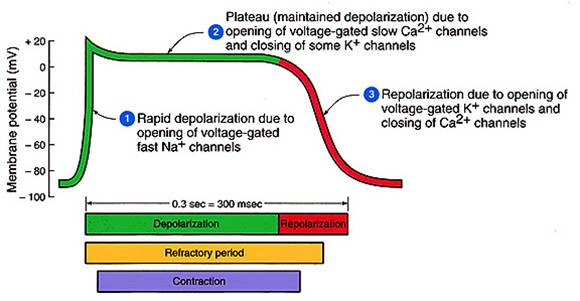
\includegraphics[width=\linewidth]{potential}
\end{figure}
\end{frame}

\begin{frame}[fragile]{Effect of chemicals, temperature, ions}
\begin{itemize}
\item Heart rate can be modulated by varying the temperature, ions
\item Chemicals also affect by inhibiting/mimicing/enhancing the action of organic chemicals such as acetylcholine
\item Temperature may or may not have an effect
\item $NA^+$, $K^+$ decrease the strength of contraction, $Ca^{+2}$ increases
\end{itemize}
\end{frame}

\begin{frame}[fragile]{Signup for presentations}
\begin{itemize}
\item Presentations: Week of 17th, 24th, 31st October
\item Sign-up with your topics
\item 10 minute presentation followed by Q \& A on topic of your choice
\item Topic needs to pertain to physiology/biology
\item Examples: Pancreatic cancer, muscular diseases etc.
\item Sign-ups on first come basis.
\end{itemize}
\end{frame}

\begin{frame}[fragile]{Office Hours}
\begin{center}
No office hours next week.
\end{center}

\Large \begin{center}Tuesday: 9-10AM\\
Thursday: 9-10AM\\
ZSH 372\\
\vspace*{2cm}
Saket Choudhary\\ 
skchoudh@usc.edu\\
\end{center}


\end{frame}

\end{document}
